\documentclass{article}
\usepackage[polish]{babel}
\usepackage[T1]{fontenc}
\usepackage{geometry}
\usepackage{chngpage}
\usepackage{graphicx}
\usepackage{subcaption}
\usepackage{algorithm2e}
\usepackage{amsfonts}
\graphicspath{ {./plots/} }
\geometry{margin=2cm}
\usepackage[utf8]{inputenc}
\usepackage{indentfirst}
\usepackage{longtable}
\author{Nie interesuj się}
\title{\vspace{-2.0cm}Sprawozdanie}
\frenchspacing
\setlength{\parindent}{2em}
\begin{document}
\maketitle
\section*{Ilorazy Różnicowe}
\noindent \textbf{Opis : }\\\\
Celem jest zaimplementowanie funkcji \textit{'ilorazyRoznicowe'} obliczającej ilorazy różnicowe w oparciu o podane węzły i odpowiadające im wartości funkcji. Dodatkowym wymaganiem był algorytm zoptymalizowany dla pamięci.\\\\
Iloraz różnicowy N-tego rzędu oblicza się za pomocą wzoru rekurencyjnego\\\\
dla k = 0:
$$f[x_i] = f(x_i),\hspace*{0,2cm} (0 \leq i \leq N)$$
dla k = 1:
$$f[x_i,x_j] = \frac{f(x_j)-f(x_i)}{x_j - x_i}$$
dla k > 1:
$$f[x_i,x_{i+1},...,x_{i+k}] = \frac{f[x_{i+1},x_{i+2},...,x_{i+k})-f(x_i,x_{i+1},...,x_{i+k-1}]}{x_{i+k} - x_i}, \hspace*{0,2cm} (0 \leq i \leq i+k \leq N)$$
\noindent \textbf{Działanie algorytmu : }\\\\
Dzięki znajomości węzłów $x_i$ oraz wartości funkcji $f(x_i)$ jesteśmy w stanie stworzyć tablicę ilorazów różnicowych wyższych rzędów:
$$przyjmujemy : \hspace*{0,2cm} c_{ik} = f[x_i,x_{i+1},...,x_{i+k}],\hspace*{0,2cm} wtedy:$$
\begin{center}
	\begin{tabular}{p{2cm} p{2cm} p{2cm} p{2cm} p{2cm} p{2cm}}
		$c_{0,0}$ & $c_{0,1}$ & $c_{0,2}$ & $...$ & $c_{0,k-1}$ & $c_{0,k}$  \\
		$c_{1,0}$ & $c_{1,1}$ & $c_{1,2}$ & $...$ & $c_{1,k-1}$  & $ $ \\
		$...$ & $...$ & $...$ & $...$ & $ $ & $ $ \\
		$c_{k-1,0}$ & $c_{k-1,1}$ & $ $ & $ $ & $ $ & $ $  \\
		$c_{k,0}$ & $ $ & $ $ & $ $ & $ $ & $ $ \\
	\end{tabular}
\end{center}
Ogólny wzór na $c_{i,k}$ jest więc następujący:
$$c_{i,k} = \frac{c_{i+1,k-1}-c_{i,k-1}}{x_{i+k}-x_i}$$
Do stworzenia naiwnego algorytmu opartego na ww. tabeli potrzebna jest tablica dwuwymiarowa, lecz jak możemy zauważyć, jest ona nieoptymalna z punktu widzenia pamięci - używamy tylko połowy zadeklarowanej tablicy.\\
Możemy jednakże skorzystać także z jednowymiarowej tablicy $fx$:
\begin{enumerate}
	\item Na początku wartościami $fx[i]$ są $c_{i,0}=f(x_i)$ a potem $c_{i-1,1},c_{i-2,2},...,c_{0,i}$ dla każdego kolejnego wyrazu z $fx[i]$
	\item Z każdym przejściem, tworzą się kolejne kolumny z tablicy ilorazów, od dołu do góry, co zapewnia że tablica będzie zawsze zawierać ilorazy potrzebne do dalszych obliczeń.\\\\
\end{enumerate}
\noindent \textbf{Pseudokod: } \\\\
Dane:
\begin{itemize}
	\item x - wektor długości n+1 zawierający węzły
	\item f - wektor długości n+1 zawierający wartości funkcji w węzłach
\end{itemize}
Wyniki:
\begin{itemize}
	\item fx - wektor długości n+1 zawierający obliczone ilorazy różnicowe
\end{itemize}
\rule{\textwidth}{0.4pt}
\begin{algorithm}[H]
	\KwData{$x,f$}
	\KwResult{$fx$}
	\vspace{0.3cm}
	\For {$i \gets 1$ \textbf{to} $length(f)$ }{
		$fx[i] \gets f[i]$
	}
	\For{$i \gets 1$ \textbf{to} $length(f)$ }{
		\For{$j \gets length(f)$ \textbf{downto} $i$ }{
			$fx[j] \gets \frac{fx[j] - fx[j-1]}{x[j] - x[j-i]}$	
		}
	\Return{$fx$}
	}
\end{algorithm}
\hrule
\vspace{0.3cm}
\section*{Wielomian Interpolacyjny}
\noindent \textbf{Opis : }\\\\
Celem jest zaimplementowanie funkcji \textit{'warNewton'} obliczającej wartość wielomianu interpolacyjnego stopnia n, w postaci Newtona $N_n(x)$ w punkcie $x = t$ za pomocą uogólnionego wzoru Hornera. Funkcja ma działać w czasie liniowym ($O(n)$). \\\\
\noindent \textbf{Działanie algorytmu : }\\\\
Wzór na wielomian Newtona przedstawiony używając ilorazów różnicowych:
$$N_n(x) = \sum_{i=0}^{n}f[x_0,x_1,...,x_i]\prod_{j=0}^{i-1}(x-x_j)$$
Zaletą takiego przedstawienia wzoru jest fakt, że dodanie kolejnych punktów $x_i,y_i$ nie narusza w żaden sposób wcześniej obliczonych współczynników $c_k = f[x_0,x_1,...,x_k]$ (metoda jest dobrze uwarunkowana pod względem numerycznym). Dla tak wyrażonego wielomianu możemy również w łatwy sposób obliczyć jego wartość stosując uogólniony algorytm Hornera:
\begin{enumerate}
	\item $\omega_n(x) \gets f[x_0,x_1,...,x_n] $
	\item $\omega_k(x) \gets \omega_{k+1}(x-x_k)+f[x_0,x_1,...,x_l] \hspace{0.2cm} (k=n-1,n-2,...,0)$
	\item $N_n(x)= \omega_0(x)$\\\\
\end{enumerate}
\noindent \textbf{Pseudokod: } \\\\
Dane:
\begin{itemize}
	\item x - wektor długości n+1 zawierający węzły
	\item fx - wektor długości n+1 zawierający wartości funkcji w węzłach
	\item t - punkt w którym będziemy liczyć wartość wielomianu 
\end{itemize}
Wyniki:
\begin{itemize}
	\item nt - wartość wielomianu w punkcie $t$
\end{itemize}
\rule{\textwidth}{0.4pt}
\begin{algorithm}[H]
	\KwData{$x,fx, t$}
	\KwResult{$nt$}
	\vspace{0.3cm}
	$n \gets length(fx)$\\
	$nt \gets fx[n]$\\
	\For {$i \gets n-1$ \textbf{downto} $1$ }{
		$nt \gets fx[i]+ (t-x[i])*nt$
	}
	\Return{$nt$}
\end{algorithm}
\hrule
\vspace{0.3cm}
\section*{Postać naturalna}
\noindent \textbf{Opis: } \\\\
Celem jest zaimplementowanie algorytmu (funkcja \textit{'naturalna'}) obliczającego współczynniki $a_0,a_1,...,a_n$ postaci naturalnej wielomianu interpolacyjnego dla zadanych współczynników $c_0=f[x_0],c_1=f[x_0,x_1],...,c_n=f[x_0,...,x_n]$ tego wielomianu w postaci Newtona oraz węzłów $x_0,...,x_n$, w czasie ($O(n^2)$).\\\\
\noindent \textbf{Działanie algorytmu: } \\\\
Aby znaleźć współczynniki wielomianu interpolacyjnego w postaci naturalnej, zastosowałem uogólniony algorytm Hornera z zadania poprzedniego. Zasada działania opracowanego na tej postawie algorytmu jest następująca:
\begin{enumerate}
	\item W wielomianie interpolacyjnym n-tego stopnia współczynnik $a_n$ przy najwyższej potędze $x$ jest równy $c_n$. Wynika z tego że $\omega_n$ jest również równy $a_n$.
	\item Mając $\omega_n = a_n$, w kolejnych krokach algorytmu tworzone są wartości $a_i$ bazujące na $a_{i+1}$.
	\item Aby znaleźć zależności między kolejnymi $a_i$, algorytm przechodzi po każdym $\omega_i$ od $i=n$ do $i = 0$, zmieniając tworzone współczynniki postaci naturalnej, tak by doprowadzić do postaci naturalnej.
\end{enumerate}
\noindent \textbf{Pseudokod: } \\\\
Dane:
\begin{itemize}
	\item x - wektor długości n+1 zawierający węzły
	\item fx - wektor długości n+1 zawierający wartości funkcji w węzłach
\end{itemize}
Wyniki:
\begin{itemize}
	\item a - wektor dlugośc n+1, zawierający obliczone współczynniki postaci naturalnej
\end{itemize}
\rule{\textwidth}{0.4pt}
\begin{algorithm}[H]
	\KwData{$x,fx$}
	\KwResult{$a$}
	\vspace{0.3cm}
	$n \gets length(fx)$\\
	$a[n] \gets fx[n]$\\
	\For {$i \gets n-1$ \textbf{downto} $0$ }{
		$a[i] \gets fx[i]- x[i]*a[i+1]$\\
		\For {$j \gets i+1$ \textbf{to} $n-1$ }{
		$a[j] \gets a[j] - x[j]*a[j+1]$
		}
	}
	\Return{$a$}
\end{algorithm}
\hrule
\vspace{0.3cm}
\newpage
\section*{Interpolacja funkcji oraz wykres}
\noindent \textbf{Opis: } \\\\
Celem jest zaimplementowanie funkcji \textit{'rysujNnfx'} intepolującej zadaną funkcję $f$ w przedziale $[a,b]$ za pomocą wielomianu intepolacyjnego $n$ w postaci Newtona, oraz rysującej wykresy funkcji $f$ i otrzymanego wielomianu. Przy interpolacji należało użyć węzłów równoodległych.\\\\
\noindent \textbf{Działanie : } 
\begin{enumerate}
	\item Wyznaczane są węzły interpolacji $(x_1,x_2,...,x_{n+1})$, które rozmieszczone są równomiernie w odległości $\frac{b-a}{n}$ (równoodległe), oraz wyznaczana jest wartość funkcji $f$ we wskazanych węzłach.
	\item Za pomocą funkcji \textit{ilorazyRoznicowe} obliczane są ilorazy różnicowe dla wskazanych wcześniej węzłów.
	\item Dla zwiększenia dokładności wykresów, zarówno funkcja $f$ jak i wielomian są próbkowane w $30*(n+1)$ równoodległych punktach. Wartości wielomianu w tych punktach są obliczone za pomocą funkcji \textit{warNewton}.
	\item Uzyskane w ten sposób wartości są wystarczające do stworzenia wykresu funkcji $f$ oraz jej wielomianu interpolacyjnego. Do rysowania wykresów użyte zostały bibliteki \textit{Plots} oraz \textit{SymPy}.
\end{enumerate}
\noindent \textbf{Pseudokod: } \\\\
Dane:
\begin{itemize}
	\item f - zadana funkcja
	\item a - początek przedziału interpolacji
	\item b - koniec przedziału interpolacji
	\item n - stopień wielomianu
\end{itemize}
Wyniki:
\begin{itemize}
	\item plik.png - wykres funkcji i jej wielomianu interpolacyjnego
\end{itemize}
\rule{\textwidth}{0.4pt}
\begin{algorithm}[H]
	\KwData{$f,a,b,n$}
	\KwResult{$a$}
	\vspace{0.3cm}
	$x,y,fx \gets array[n+1]$\\
	$density \gets 30$\\
	$w\_x,w\_y,w\_n \gets array[(n+1)*density]$\\
	$max\_w \gets n+1$\\
	$h \gets \frac{(b-a)}{n}$\\
	$k\_h \gets 0.0$  //kolejne wartości h\\
	\For {$i \gets 1$ \textbf{to} $max\_w$ }{
		$x[i] \gets a+k\_h$\\
		$y[i] \gets f(x[i])$\\
		$k\_k \gets k\_h + h$\\
	}
	$fx \gets ilorazyRoznicowe(x,y)$\\
	
	$k\_h \gets 0.0$\\
	$max\_w \gets max\_w * density$\\
	\For {$i \gets 1$ \textbf{to} $max\_w$ }{
		$w\_x[i] \gets a + k\_h$\\
		$w\_y[i] \gets f(w\_x[i])$\\
		$w\_n[i] \gets warNewton(x,fx,w\_x[i])$\\
		$k\_h \gets k\_h + h$\\
	}
	$draw(w\_x,w\_y,w\_n)$
\end{algorithm}
\hrule
\section*{Interpolacja funkcji $e^x$ oraz $x^2*sinx$}
\noindent \textbf{Opis: } \\\\
Zastosowanie funkcji \textit{rysujNnfx} na następujących przykładach:
\begin{itemize}
	\item $f(x) = e^x$, $[a,b] = [0,1]$, $n \in \{5,10,15\}$
	\item $f(x) = x^2*sinx$, $[a,b] = [-1,1]$, $n \in \{5,10,15\}$
\end{itemize}

\noindent \textbf{Wyniki: }
\begin{figure}[ht]
	\begin{subfigure}{.5\textwidth}
		\centering
		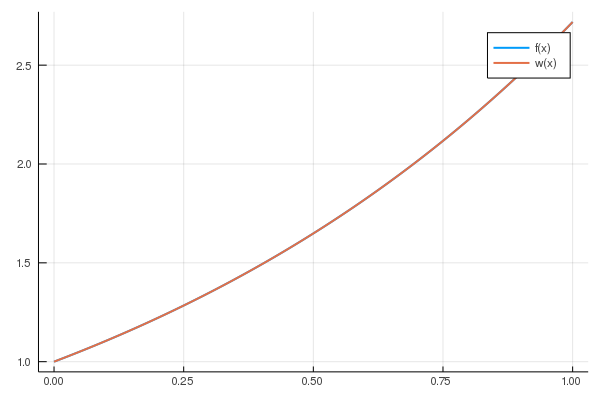
\includegraphics[width=.8\linewidth]{plots/5_1.png}  
		\caption*{$f(x) = e^x$, n = 5}
	\end{subfigure}
	\begin{subfigure}{.5\textwidth}
		\centering
		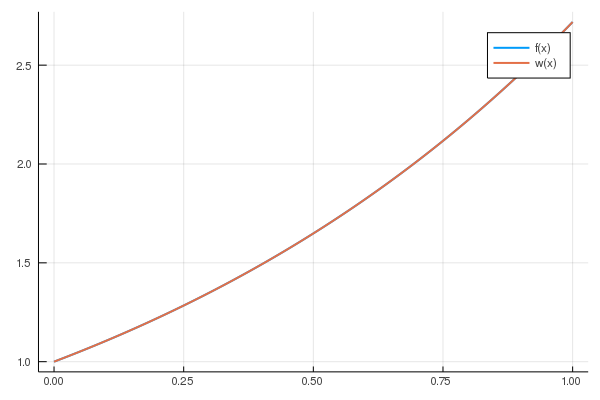
\includegraphics[width=.8\linewidth]{plots/5_2.png}  
		\caption*{$f(x) = e^x$, n = 10}
	\end{subfigure}
\end{figure}
\begin{figure}[ht]
	\begin{subfigure}{.5\textwidth}
		\centering
		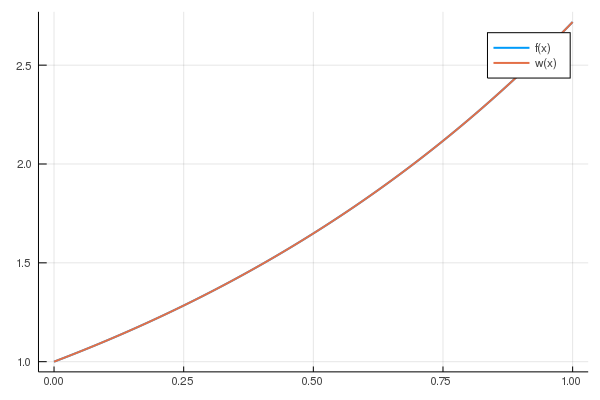
\includegraphics[width=.8\linewidth]{plots/5_3.png}  
		\caption*{$f(x) = e^x$, n = 15}
	\end{subfigure}
	\begin{subfigure}{.5\textwidth}
		\centering
		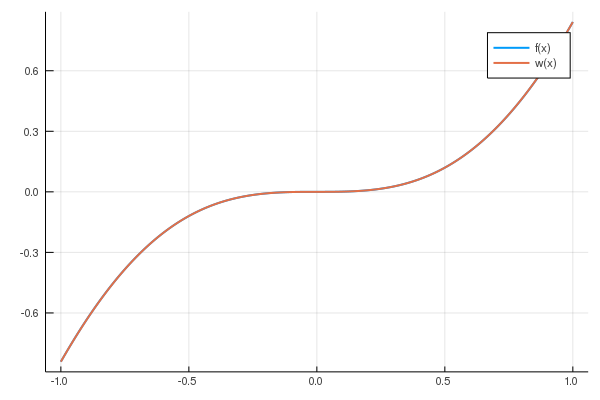
\includegraphics[width=.8\linewidth]{plots/5_4.png}  
		\caption*{$f(x) = x^2*sinx$, n = 5}
	\end{subfigure}
\end{figure}
\begin{figure}[ht]
	\begin{subfigure}{.5\textwidth}
		\centering
		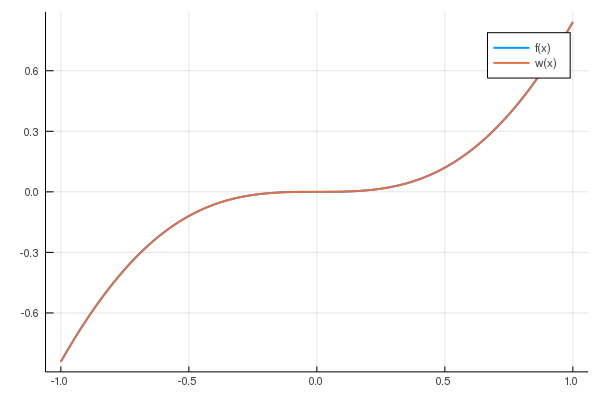
\includegraphics[width=.8\linewidth]{plots/5_5.png}  
		\caption*{$f(x) = x^2*sinx$, n = 10}
	\end{subfigure}
	\begin{subfigure}{.5\textwidth}
		\centering
		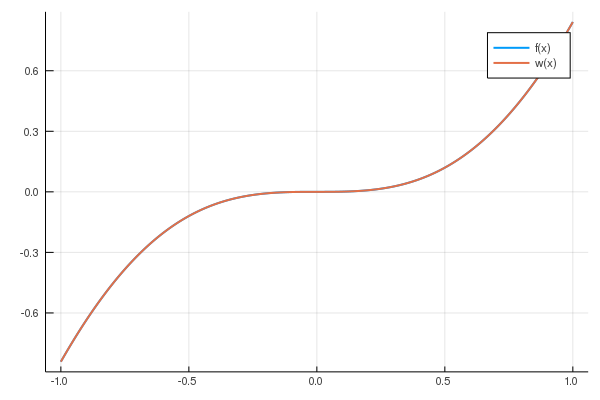
\includegraphics[width=.8\linewidth]{plots/5_6.png}  
		\caption*{$f(x) = x^2*sinx$, n = 15}
	\end{subfigure}
\end{figure}\\\\
\newpage
\noindent \textbf{Wnioski: } \\\\
Dla obu funkcji, na zadanych przedziałach wielomiany interpolacyjne są bardzo bliskie interpolowanym funkcjom, na żadnym z wykresów nie widać rozbieżności. W tym przypadku zastosowanie równoodległych węzłów interpolacji dało bardzo dobre przybliżenia funkcji interpolowanych.

\section*{Interpolacja funkcji $|x|$ oraz $\frac{1}{1+x^2}$}
\noindent \textbf{Opis: } \\\\
Zastosowanie funkcji \textit{rysujNnfx} na następujących przykładach:
\begin{itemize}
	\item $f(x) = |x|$, $[a,b] = [1-,1]$, $n \in \{5,10,15\}$
	\item $f(x) = \frac{1}{1+x^2}$, $[a,b] = [-5,5]$, $n \in \{5,10,15\}$
\end{itemize}
\noindent \textbf{Wyniki: }
\begin{figure}[ht]
	\begin{subfigure}{.5\textwidth}
		\centering
		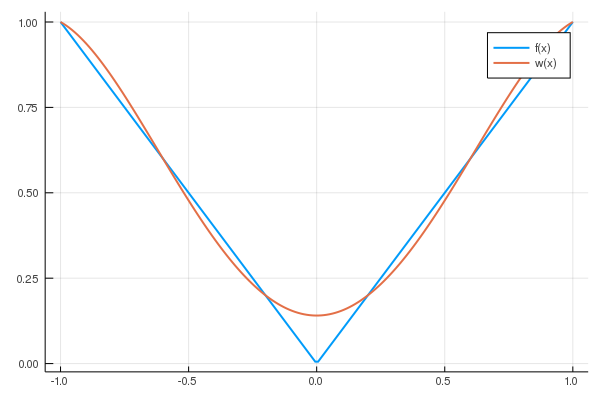
\includegraphics[width=.8\linewidth]{plots/6_1.png}  
		\caption*{$f(x) = |x|$, n = 5}
	\end{subfigure}
	\begin{subfigure}{.5\textwidth}
		\centering
		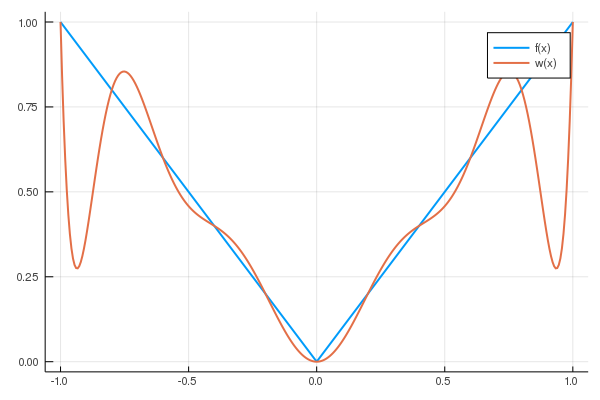
\includegraphics[width=.8\linewidth]{plots/6_2.png}  
		\caption*{$f(x) = |x|$, n = 10}
	\end{subfigure}
\end{figure}
\begin{figure}[ht]
	\begin{subfigure}{.5\textwidth}
		\centering
		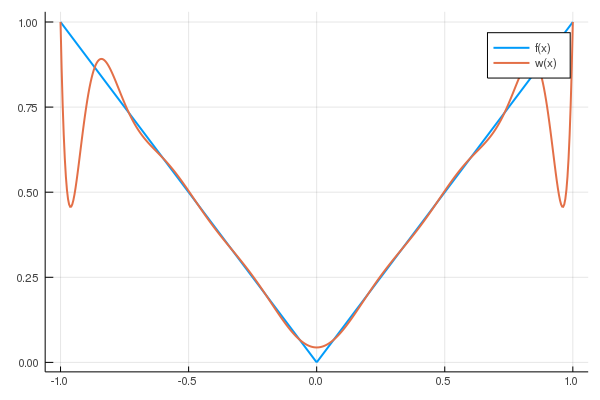
\includegraphics[width=.8\linewidth]{plots/6_3.png}  
		\caption*{$f(x) = |x|$, n = 15}
	\end{subfigure}
	\begin{subfigure}{.5\textwidth}
		\centering
		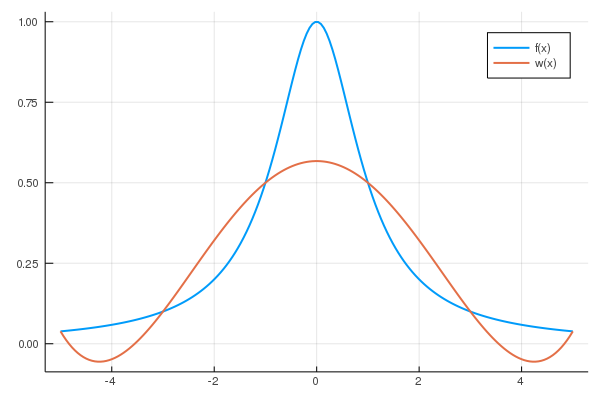
\includegraphics[width=.8\linewidth]{plots/6_4.png}  
		\caption*{$f(x) = \frac{1}{1+x^2}$, n = 5}
	\end{subfigure}
\end{figure}
\begin{figure}[ht]
	\begin{subfigure}{.5\textwidth}
		\centering
		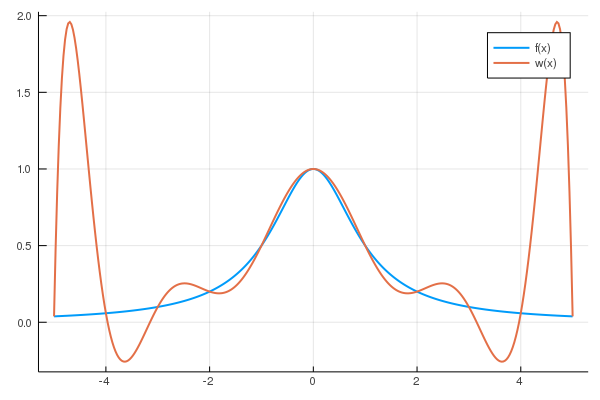
\includegraphics[width=.8\linewidth]{plots/6_5.png}  
		\caption*{$f(x) = \frac{1}{1+x^2}$, n = 10}
	\end{subfigure}
	\begin{subfigure}{.5\textwidth}
		\centering
		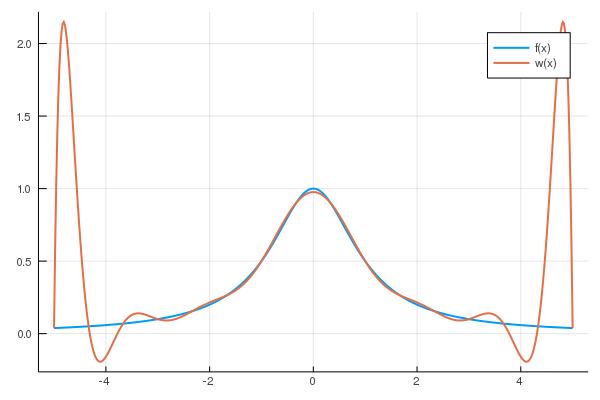
\includegraphics[width=.8\linewidth]{plots/6_6.png}  
		\caption*{$f(x) = \frac{1}{1+x^2}$, n = 15}
	\end{subfigure}
\end{figure}\\\\
\newpage
\noindent \textbf{Wnioski: } \\\\
Dla obu przypadków obserwujemy wyraźne rozbieżności, szczególnie dla końców przedziału.
\begin{itemize}
	\item Funkcja $|x|$ nie jest różniczkowalna, co w największym stopniu dopwiada za odchylenia w tym przypadku.
	\item Dla funkcji $\frac{1}{1+x^2}$ obserwujemy \textit{efekt Runge'go} - pogorszenie jakości interpolacji wielomianowej, mimo zwiększenia ilości węzłów. Jest to typowe zjawisko dla przypadku gdy węzły wielomianu są równoodległe, a sam wielomian jest wysokiego stopnia, co powoduje znaczne odchylenia wartości wielomianu od wartości funkcji na końcach badanym przedziale. Efekt występuje również, gdy badana funkcja jest nieciągła, lub odbiega znacząco do funkcji gładkiej.
\end{itemize}
Głónym czynnikiem, który wpływa na niską dokładność powyższych przybliżeń, jest fakt równoodległości węzłów, przez co w miejscu o trudniejszej interpolacji przypada ich stosunkowo niewiele. Uniwersalnym sposobem na poprawę interpolacji w ww. przypadkach jest stosowanie wielomianów opartych na węzłach Czebyszewa, które dzięki oparciu na węzłach mocno zagęszczonych przy końcach przedziałów mają znacznie mniejsze oscylacje. W celu najdokładniejszego przybliżenia funkcji, należy dobrać węzły w sposób otymalny (na przykład stosując zera wielomianu Czebyszewa).
\end{document}










